\section{Pitfalls of Performant High Level Language Runtimes}\label{chpt:1:sec:1}

The evolution of computational science has been marked by the introduction and adoption of high-level interpreted languages that are designed to be user friendly, and cross platform. Starting with Matlab in the 1970s, followed by Python in the 1990s, and more recently Julia in the 2010s. High-level languages have significantly impacted scientific computing, offering efficient implementations of algorithms and introducing optimised data structures via projects such as NumPy and SciPy, as well as ergonomic cross platform build systems. While these languages facilitate easier experimentation, achieving peak performance often necessitates manual memory management or explicit instruction set level programming to ensure vectorisation on a given hardware target. A natural question for us when deciding on a programming environment for this project was whether advancements in high-level languages were sufficient for the implementation of `fast algorithms'. If they proved to be sufficient our software would be free of the so called `two language' problem, in which a user friendly interfaces in a high-level language provides a front-end for a compiled language implementation of more data-intensive operations. This problem plagues academic software development, as resulting software relies on a brittle low-level interface between the high-level front-end, and low-level back-ends for performance critical code sections.

Recent strategies to enhance the performance of high-level languages have involved refining compiler technology. These projects are advertised as tools that allow developers to use high-level languages for quick algorithm experimentation, while leaving it to the compiler to produce efficient machine code. Benchmarks are usually offered with respect certain numerical operations that can be vectorized, such as iteration over aligned data structures, with compilers taking care to unroll loops and apply inlining to inner function calls.

Noteworthy examples are the Numba project for Python and the Julia language. Both leverage the LLVM compiler infrastructure, which aims to standardise the back-end generation of machine code across various platforms. This approach, known as `just in time' (JIT) compilation, generates code at runtime from the types of a function's signature. Figure \ref{fig:chpt:1:sec:1:numba_runtime} provides a sketch of how Numba in particular generates machine code from high-level Python code. The LLVM compiler supports numerous hardware and software targets, including platforms like Intel and Arm, and provides multithreading through support for compiler extensions such as OpenMP. Additionally, these compilers offer native support for GPU code generation. An important difference between Numba and Julia is that Numba is simply a compiler built to optimise code written for the numerical types created using the NumPy library, and Julia is a fully fledged language. Numba contains implementations of algorithms for a subset of the scientific Python ecosystem, specifically functionality from the NumPy project for array manipulation and linear algebra.

As many performance benchmarks for these programming environments are typically provided for algorithms that rely on simpler data structures, we decided to test these high-level environments for more complex algorithms before making a choice about our programming environment for this project. We implemented a single node multi-threaded FMM using Python's Numba compiler, identifying two notable pitfalls with this approach, the full results of which were recently published in Computing in Science and Engineering \cite{kailasa2022pyexafmm}.

Firstly, JIT compilation of code imposes a significant runtime cost that is disruptive to development. Compiled functions are by default not cached between interpreter sessions in either Julia or Numba code. Our FMM code takes $15 \pm 1$s to compile when targeting a i7-9750H CPU with x86 architecture, where the benchmark is given with respect to seven runs. This is comparable to the runtime of the FMM software for a typical benchmark FMM problem \footnote{1e6 particles distributed randomly, using order $p=6$ expansions for a Laplace problem takes approximately 30s on this hardware using our software. See Chapter \ref{chpt:2:designing_software_for_fast_algorithms} for more details on the FMM and the significance of these terms.}. For smaller problem sizes, the compilation time dominates runtime. Ahead of time (AOT) compilation is partially supported in Numba, and can be used to build binaries for distribution to different hardware targets, e.g. x86 or ARM. However support for AOT compiled code is currently second class, the machine code created in this manner are usable only from the Python interpreter and not from within calls made from other Numba compiled functions, and it's currently staged for deprecation and replacement. We note that Julia does support AOT compilation via the PackageCompiler.jl module. This allows for different levels of AOT compilation, from creating a `sysimage' which amounts to a serialised file containing the compiled outputs of a Julia session, a `relocatable app' which includes an executable compiled to a specific hardware target alongside Julia itself, to creating a C library which can be precompiled for a specific hardware target such as x86. However, this requires relatively advanced software engineering skills, and raises the barrier to entry for high-performance computing with Julia.

Thus switching to such a programming environment requires developers to create a workflow that keeps interpreter sessions active for as long as possible in order to reduce the impact of long compilation times, or write build scripts for AOT compilation for a specific hardware target similar to compiled languages. As one of the key advantages of high-level languages is their developer friendliness and simple build systems this acts as an impediment.

Downstream users of software, who may also be using JIT compilers for their own code, are faced with significant compilation times, and potentially intricate build steps unless catered for by the original library's developers. This problem compounds in the case of distributed memory programs using MPI, as JIT compilation imposes runtime costs to the entire program. Unless a project has been distributed as a binary, by default MPI runs are not interactive, and therefore require a recompilation for each run. This isn't to say MPI programs written in Julia or Numba haven't been scaled to large HPC systems, however their usage does carry a cost in terms of developer workflow, and potentially program runtime.

Secondly, our experience in developing the FMM in Numba made clear how difficult it can be to anticipate the behaviour of Numba when considering how to optimise functions with different implementations of the same logic. Consider the code in Listing \ref{code:chpt:1:sec:1:numba_compiler_optimisations}, here we show three logically equivalent ways of performing two matrix-matrix products, and storing a column from the result in a dictionary. A dictionary is chosen for storage as this mirrors the data structure used in our FMM software for storing intermediate results. The runtimes of all three implementations are shown in Table \ref{table:chpt:1:sec:1:numba_compiler_optimisations} for different problem sizes. We choose this example because this operation of matrix-matrix multiplication is well supported by Numba, and data instantiation, whether from within or external to a Numba compiled function, should in principle make little difference as the Numba runtime simply dereferences pointers to heap allocated memory when entering a Numba compiled code segment. This example is designed to illustrate how arbitrary changes to writing style can impact the behavior of Numba code. The behavior is likely due to the initialisation of a dictionary from within a calling Numba function, rather than an external dictionary, and having to return this to the user. However, the optimisations taken by Numba are presented opaquely to a user and it's unclear why there are performance variations at all.

In developing our FMM code we faced significant challenges in tweaking our code and data structures to maximise the performance achieved from within Numba. From manually inlining subroutines as in Listing \ref{code:chpt:1:sec:1:numba_compiler_optimisations}, to testing where to allocate data. Our final code took a significant amount of time to develop, approximately six months, and was organised in a manner that optimised for performance rather than readability. Thus, despite being a \textit{compiler} for numerical Python, Numba behaves in practice more like a \textit{programming framework} which a developer had to adhere to strictly in order to achieve the highest level of performance. The disadvantage of this is that the framework is both relatively restrictive, but also presented opaquely to a user.

Therefore, while being a technology with great features, Numba was not decided to be a suitable choice for our programming environment. Its ability to target a diverse set of hardware targets from Python, leveraging the power of LLVM to write multithreaded, and autovectorised code, as well as writing CPU and GPU code from within Python, while allowing downstream projects to develop in a familiar language with a large open-source ecosystem and simple dependency management demonstrate the utility of this remarkable tool. However, the constraints of high level languages, specifically the inability to manage memory at a system level, as well as the development costs of JIT compilation, and Numba's framework-like behaviour demonstrate that while being useful, it is preferable to write our software platform using a systems-level language where high-performance can be assumed. Our criticisms of Numba also apply to Julia. However we note that Julia has certain advantages over Numba including its design and syntax focussed on mathematical computing, native support for multithreading, a richer type system and a large open-source community with a scientific computing focus.

System level languages have progressed commensurately to high-level languages in recent decades. Modern languages such as Go and Rust, offer runtimes with informative compilers, inbuilt documentation and testing facilities, as well as LLVM backends to support code generation across platforms, removing much of the complexity associated with building and distributing software written in C/C++. Rust in particular, uninhibited by a garbage collector as for Go, makes it easy to interoperate Rust code with libraries built in C/C++ via its foreign function interface, making it simple to leverage existing open-source scientific software.  We therefore conclude that the two language problem is minimised in comparison to the past, and modern system level programming languages potentially offer an effective solution for building academic software.

\begin{figure}[h]
    \centering
    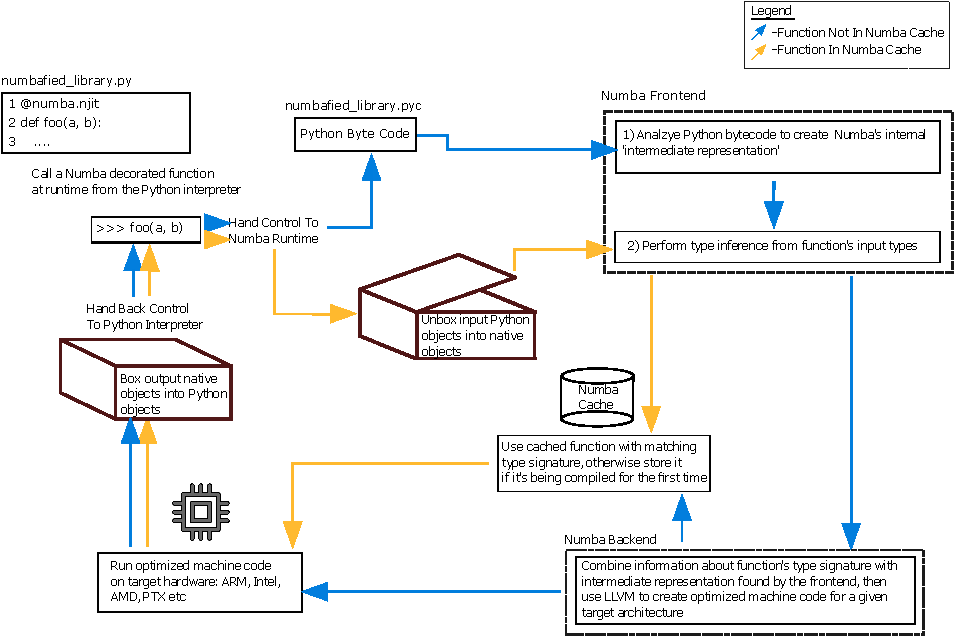
\includegraphics[width=\linewidth]{images/ch_1/numba.pdf}
    \caption{A visualisation of the Numba runtime system. A function decorated with `njit' acts as an instruction to the runtime to check a database for any Numba-compiled functions with a matching function signature, if this doesn't exist Numba generates a new compiled function and caches it using LLVM. Future calls of this function use this cached version in place of the Python interpreter. Code relies on Numba's runtime to correctly `box' and `unbox' native Python objects into data structures compatible with Numba code, which operates on a subset of numerical data structures created using the NumPy library. Figure adapted from \cite{kailasa2022pyexafmm}.}
    \label{fig:chpt:1:sec:1:numba_runtime}
\end{figure}


\pagebreak

% \begin{figure}[H]
\begin{lstlisting}[language=Python, caption={Three ways of writing a trivial algorithm in Numba, that performs some computation and saves the results to a dictionary. Adapted from Listing 2 in \cite{kailasa2022pyexafmm}},  label=code:chpt:1:sec:1:numba_compiler_optimisations]
import numpy as np
import numba
import numba.core
import numba.typed

# Initialise in the Python interpreter
data = numba.typed.Dict.empty(
    key_type=numba.core.types.unicode_type,
    value_type=numba.core.types.float64[:]
)

data['initial'] = np.ones(N)

# Subroutine 1
@numba.njit
def step_1(data):
    """
    Initialise a matrix and perform a matrix matrix product,
    storing a single column in the data dictionary.
    """
    a = np.random.rand(N, N)
    data['a'] = (a @ a)[0,:]


# Subroutine 2
@numba.njit
def step_2(data):
    """
    Initialise a matrix and perform a matrix matrix product,
    storing a single column in the data dictionary.
    """
    b = np.random.rand(N, N)
    data['b'] = (b @ b)[0,:]


@numba.njit
def algorithm_1(data):
    """
    First implementation.
    """
    step_1(data)
    step_2(data)


@numba.njit
def algorithm_2(data):
    """
    Second implementation.
    """
    # This time the storage dictionary is created within the
    # Numba function, so the types are inferred by the Numba
    # runtime, this also avoids a boxing cost to create a Numba
    # type from a Python one.
    data = dict()
    data['initial'] = np.ones(N)
    step_1(data)
    step_2(data)
    return data

@numba.njit
def algorithm_3(data):
    """
    Third implementation.
    """

    # This time, the subroutines are manually inlined
    # by the implementer, as well as the initialisation
    # of the results dictionary locally, as in algorithm_2.

    data = dict()
    data['initial'] = np.ones(N)

    def step_1(data):
        a = np.random.rand(N, N)
        data['a'] = (a @ a)[0,:]


    # Subroutine 2
    @numba.njit
    def step_2(data):
        b = np.random.rand(N, N)
        data['b'] = (b @ b)[0,:]

    step_1(data)
    step_2(data)
    return data
\end{lstlisting}
% \end{figure}
% \afterpage{\clearpage}


\begin{table}
    \centering
    \caption{Performance of different algorithms from Listing \ref{code:chpt:1:sec:1:numba_compiler_optimisations}, taken on an i7 CPU and averaged over seven runs for statistics.}
    \begin{tabular}{l l l}
        \toprule
        Algorithm & Matrix dimension & Time ($\mu s$) \\
        \midrule
        1 & \(\mathbb{R}^{1 \times 1}\) & 1.55 $\pm$ 0.01 \\
        1 & \(\mathbb{R}^{100 \times 100}\) & $304 \pm 3$\\
        1 & \(\mathbb{R}^{1000 \times 1000}\) & $29,100 \pm 234$ \\
        \midrule
        1 & \(\mathbb{R}^{1 \times 1}\) & $2.73 \pm 0.01$ \\
        1 & \(\mathbb{R}^{100 \times 100}\) & $312 \pm 3$ \\
        1 & \(\mathbb{R}^{1000 \times 1000}\) & $25,700 \pm 92$ \\
        \midrule
        1 & \(\mathbb{R}^{1 \times 1}\) & $2.71 \pm 0.01$ \\
        1 & \(\mathbb{R}^{100 \times 100}\) & $312 \pm 1$ \\
        1 & \(\mathbb{R}^{1000 \times 1000}\) & $25,700 \pm 140$ \\
        \bottomrule
    \end{tabular}
    \label{table:chpt:1:sec:1:numba_compiler_optimisations}
\end{table}
